\documentclass{beamer}
\usetheme{CambridgeUS}

\usepackage{tikz}

\usepackage[croatian]{babel}
\usepackage[utf8x]{inputenc}
\usepackage[T1]{fontenc}
\usepackage[autostyle]{csquotes}
\usepackage{amsmath}
\usepackage{url}
\usepackage{fancybox}
\usepackage{wasysym}
\usepackage{listings}
\usepackage{multirow}
\usepackage{pgfplots}

\newcommand{\A}[1]{#1&\texttt{\string#1}\hspace*{1ex}}

\usetikzlibrary{arrows,shapes,positioning,spy,calc,plotmarks,quotes,angles,babel}

\hypersetup{plainpages=false,bookmarksopen,linkcolor=violet,%
pdfpagemode=FullScreen,colorlinks=true%
}
\hypersetup{pdftitle={TikZ}}
\hypersetup{baseurl={http://www.math.hr}}
\hypersetup{pdfsubject={LaTeX}}
\hypersetup{pdfauthor={Ivica Nakić}}

\lstset{language=[LaTeX]TeX,extendedchars=true,backgroundcolor=\color{gray!20},identifierstyle=,stringstyle=\rmfamily,%
columns=flexible,showstringspaces=false,keywordstyle=\color{violet}\bfseries}

\lstset{literate=%
{Š}{{\v{S}}}1
{Đ}{{\Dj{}}}1
{Č}{{\v{C}}}1
{Ć}{{\'C}}1
{Ž}{{\v{Z}}}1
{š}{{\v{s}}}1
{đ}{{\dj{}}}1
{č}{{\v{c}}}1
{ć}{{\'c}}1
{ž}{{\v{z}}}1
}

\title{\LaTeX{} --- Ti\emph{k}Z}
\subtitle{}
\author{Ivica Nakić \\ \texttt{nakic@math.hr}}
\institute[PMF--MO]{Matematički odsjek Prirodoslovno--matematičkog fakulteta}
\date[2014/15]{Matematički software, 2014/15}


\begin{document}

\begin{frame}
  \maketitle  
\end{frame}

\begin{frame}[fragile]
\frametitle{Uvod u PGF/Ti\emph{k}Z}
    
PGF/Ti\emph{k}Z je tandem jezika za kreiranje vektorske grafike iz geomtrijskog/algebarskog opisa. Odnos PGF/Ti\emph{k}Z je analogan odnosu \TeX/\LaTeX. Mi ćemo se uglavnom baviti s Ti\emph{k}Zom. 
\begin{block}{}
Ti\emph{k}Z je skraćenica od \guillemotleft Ti\emph{k}Z ist \emph{kein} Zeichenprogramm\guillemotright. 
\end{block}
Dvije osnovne naredbe su \textcolor{violet}{\textbackslash tikz} i okolina \textcolor{violet}{tikzpicture}. \textcolor{violet}{\textbackslash tikz} služi za crtanje objekata gdje pripadni kod ne pralazi jedan redak. Npr.\ \tikz \fill[orange] (1ex,1ex) circle (1ex); sam dobio na korištenjem sljedećeg k\^oda:
\begin{lstlisting}
	 \tikz \fill[orange] (1ex,1ex) circle (1ex);
\end{lstlisting}
\textcolor{violet}{tikzpicture} je okolina za crtanje kompliciranijih objekata. 
\end{frame}

\begin{frame}[fragile]
\frametitle{\textcolor{violet}{tikzpicture}}
\begin{columns}
\column{4.5cm}
Ova slika \\
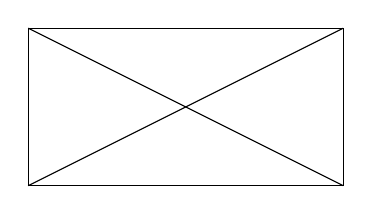
\begin{tikzpicture}
\draw (0,0) rectangle (4,2); 
\draw (0,0) -- (4,2);
\draw (0,2) -- (4,0); 
\end{tikzpicture}  
\column{5cm}
je nacrtana pomoću sljedećeg k\^oda: 
\begin{lstlisting}
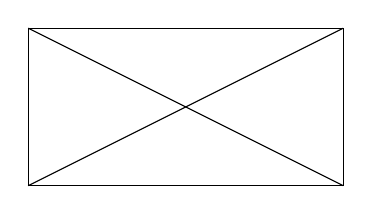
\begin{tikzpicture}
\draw (0,0) rectangle (4,2); 
\draw (0,0) -- (4,2);
\draw (0,2) -- (4,0); 
\end{tikzpicture}  
\end{lstlisting}
\end{columns}
\pause
\begin{itemize}
	\item Slika se uvijek nalazi u najmanje mogućem pravokutniku.
	\item Ukoliko ne pišu jedinice, koordinate su u centimetrima.
	\item Koordinata $(0,0)$ odgovara lijevom donjem kutu slike.
  \item Možete koristiti i polarne koordinate, format je $(\phi\colon r)$
\end{itemize}
\end{frame}

\begin{frame}[fragile]
\frametitle{Pomoćne linije (grids)}
\begin{center}
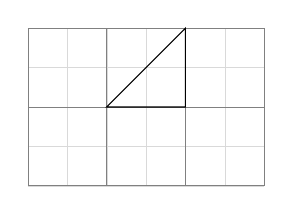
\begin{tikzpicture}
\draw[line width=0.1pt,gray!30,step=5mm] (0,0) grid (3,2);
\draw[help lines] (0,0) grid (3,2);
\draw (1,1) -- (2,2) -- (2,1) -- cycle; 
\end{tikzpicture}	
\end{center}

\begin{lstlisting}
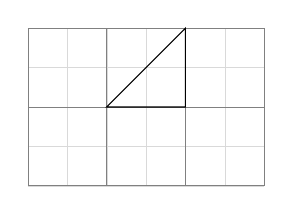
\begin{tikzpicture}
\draw[line width=0.1pt,gray!30,step=5mm] (0,0) grid (3,2);
\draw[help lines] (0,0) grid (3,2);
\draw (1,1) -- (2,2) -- (2,1) -- cycle; 
\end{tikzpicture}
\end{lstlisting} 
\begin{block}{}
U nastavku neću uvijek pisati okolinu \textcolor{violet}{tikzpicture}, pa je ne zaboravite staviti kad kopirate k\^od.
\end{block}
\end{frame}

\begin{frame}[fragile]
\frametitle{Linije}
\begin{center}
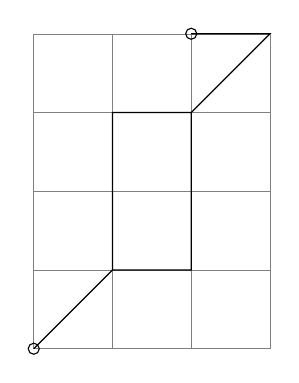
\begin{tikzpicture}
\draw[help lines] (0,0) grid (3,4); \draw (0,0) circle (2pt)
-- (1,1) rectangle (2,3) -- (3,4)
-- (2,4) circle (2pt);
\end{tikzpicture}	
\end{center}

\begin{lstlisting}
\draw[help lines] (0,0) grid (3,4); 
\draw (0,0) circle (2pt)
-- (1,1) rectangle (2,3) -- (3,4)
-- (2,4) circle (2pt);
\end{lstlisting} 
\end{frame}

\begin{frame}[fragile]
\frametitle{Davanje imena koordinatama}
Sljedeći k\^od, koji crta križani pravoutnik (%

\begin{tikzpicture}
\draw (0.0,0.0) coordinate(dolje lijevo)
-- (0.4,0.2) coordinate(upper right);
\draw (0.0,0.2) -- (0.4,0.0);
\draw (dolje lijevo) rectangle (upper right); 
\end{tikzpicture}), pokazuje kako se označavaju koordinate.	

\begin{lstlisting}
\draw (0.0,0.0) coordinate(dolje lijevo)
-- (0.4,0.2) coordinate(upper right);
\draw (0.0,0.2) -- (0.4,0.0);
\draw (dolje lijevo) rectangle (upper right); 
\end{lstlisting} 
\end{frame}

\begin{frame}[fragile]
\frametitle{(Bézierove) krivulje}
\begin{columns}
\column{4cm}
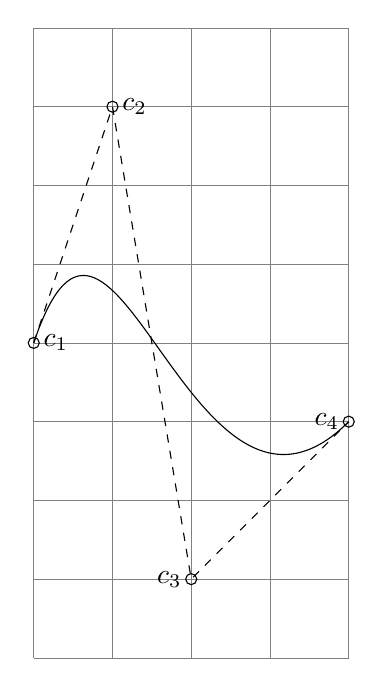
\begin{tikzpicture}
\draw[help lines] (-2,-4) grid (+2,+4); 
	\path (-2,+0) coordinate(c1)
        (-1,+3) coordinate(c2)
        (+0,-3) coordinate(c3)
        (+2,-1) coordinate(c4);
	\draw[dashed] (c1) -- (c2) -- (c3) -- (c4); 
	\draw (c1) circle (2pt)
        (c2) circle (2pt)
        (c3) circle (2pt)
        (c4) circle (2pt)
        (c1) .. controls (c2)
				and (c3) .. (c4)
(c1) node[anchor=west] {$c_1$} 
(c2) node[anchor=west] {$c_2$}
(c3) node[anchor=east] {$c_3$}
(c4) node[anchor=east] {$c_4$};
\end{tikzpicture}	
\column{5cm}
\small
\begin{lstlisting}
\draw[help lines] (-2,-4) 
grid (+2,+4); 
\path (-2,+0) coordinate(c1)
        (-1,+3) coordinate(c2)
        (+0,-3) coordinate(c3)
        (+2,-1) coordinate(c4);
\draw[dashed] (c1) -- (c2) 
-- (c3) -- (c4); 
	\draw (c1) circle (2pt)
        (c2) circle (2pt)
        (c3) circle (2pt)
        (c4) circle (2pt)
        (c1) .. controls (c2)
				and (c3) .. (c4)
(c1) node[anchor=west] {$c_1$} 
(c2) node[anchor=west] {$c_2$}
(c3) node[anchor=east] {$c_3$}
(c4) node[anchor=east] {$c_4$};
\end{lstlisting} 
\end{columns}
\end{frame}

\begin{frame}
\frametitle{Još neki primjeri}
 \tikz \draw (0,0) -- (1,1) (2,0) -- (3,0) -- (3,1) -- cycle;
 \tikz \draw (0.0,0.0) -| (2.0,0.5) (1.0,1.0) -| (3.0,0.0);     
 \tikz \draw (0.0,0.0) |- (2.0,1.0) (1.0,0.5) |- (3.0,0.0);
 \tikz \draw (0,0) rectangle (1,1) rectangle (3,2);   
 \tikz \draw (0,0) circle (2pt) rectangle (3,1) circle (4pt);
 \tikz \draw (2,2) ellipse (1cm and 1cm) (3,2) ellipse (3cm and 2cm);
\end{frame}

\begin{frame}[fragile]
\frametitle{K\^od za prethodni slajd}
\begin{lstlisting}
\tikz \draw (0,0) -- (1,1) (2,0) -- (3,0) -- (3,1) -- cycle;
\tikz \draw (0.0,0.0) -| (2.0,0.5) (1.0,1.0) -| (3.0,0.0);     
\tikz \draw (0.0,0.0) |- (2.0,1.0) (1.0,0.5) |- (3.0,0.0);
\tikz \draw (0,0) rectangle (1,1) rectangle (3,2);   
\tikz \draw (0,0) circle (2pt) rectangle (3,1) circle (4pt);
\tikz \draw (2,2) ellipse (1cm and 1cm) (3,2) ellipse (3cm and 2cm);	
\end{lstlisting}
\end{frame}

\begin{frame}[fragile]
\frametitle{Luk}
\begin{columns}
\column{3cm}
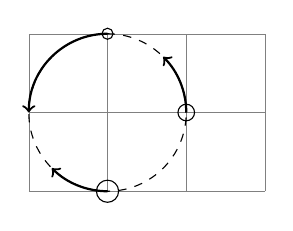
\begin{tikzpicture}
\draw[help lines] (0,0) grid (3,2); 
\draw[dashed] (1,1) circle (1cm); 
\draw (1,2) coordinate(a) circle (2pt)
      (2,1) coordinate(b) circle (3pt)
	  (1,0) coordinate(c) circle (4pt); 
\draw[->,thick] (a) arc (90:180:1cm); 
\draw[->,thick] (b) arc (0:45:1cm); 
\draw[->,thick] (c) arc (270:225:1cm); 
\end{tikzpicture}  
\column{7cm}
\begin{lstlisting}
\draw[help lines] (0,0) grid (3,2); 
\draw[dashed] (1,1) circle (1cm); 
\draw (1,2) coordinate(a) circle (2pt)
      (2,1) coordinate(b) circle (3pt)
	  (1,0) coordinate(c) circle (4pt); 
\draw[->,thick] (a) arc (90:180:1cm); 
\draw[->,thick] (b) arc (0:45:1cm); 
\draw[->,thick] (c) arc (270:225:1cm);	
\end{lstlisting}
\end{columns}  
Tri parametra naredbe \textcolor{violet}{arc} su dva kuta (u stupnjevima) te radijus kružnice na kojoj luk leži.
\end{frame}

\begin{frame}[fragile]
\frametitle{Punjenje bojom}
\begin{columns}
\column{3cm}	
\tikz \fill[blue] (0,0) rectangle (3,0.5); \\
\tikz \filldraw[fill=blue,draw=lime] 
(0,0) rectangle (3,0.5); \\
\tikz \shade[left color=white,right color=blue] 
(0,0) rectangle (3,0.5); \\
\tikz \shadedraw[left color=black,right color=white,draw=gray] 
(0,0) rectangle (3,0.5);
\column{7cm}
\begin{lstlisting}
\fill[blue] (0,0) rectangle (3,0.5);
\filldraw[fill=blue,draw=lime] 
(0,0) rectangle (3,0.5); 
\shade[left color=white,right color=blue] 
(0,0) rectangle (3,0.5);
\shadedraw[left color=black,
right color=white,draw=gray] 
(0,0) rectangle (3,0.5);	
\end{lstlisting}
\end{columns}
Neke predefinirane boje: \textcolor{black}{black}, \textcolor{blue}{blue}, \textcolor{brown}{brown}, \textcolor{cyan}{cyan}, \textcolor{darkgray}{darkgray}, \textcolor{lime}{lime}, \textcolor{magenta}{magenta}, \textcolor{olive}{olive}, \textcolor{pink}{pink}, \textcolor{teal}{teal}, \textcolor{violet}{violet}, \textcolor{yellow}{yellow}, \textcolor{orange}{orange}.

Definiranje novih boja:
\begin{lstlisting}
\definecolor{<ime>}{rgb}{<crvena>,<zelena>,<plava>} 
\definecolor{<ime>}{siva}{<omjer>} 
\colorlet{<ime>}{<boja>!<postotak>} 
\colorlet{<ime>}{<boja1>!<postotak>!<boja2>}	
\end{lstlisting}
\end{frame}

\begin{frame}[fragile]
\frametitle{Varijante korištenja boja}
\begin{columns}
\column{2cm}
\begin{tikzpicture}[color=red]
\draw (0,3) -- (2,3); 
\draw[color=green] (0,2) -- (2,2); 
\draw[color=cyan!50!red] (0,1) -- (2,1); 
\end{tikzpicture} \\
\begin{tikzpicture}[gray] 
\draw[orange!80!teal] (0,0) -- (2,0); 
\end{tikzpicture} \\
\tikz \draw[draw=gray] (0,1) -- (2,1);
\column{7cm}
\begin{lstlisting}
\begin{tikzpicture}[color=red]
\draw (0,3) -- (2,3); 
\draw[color=green] (0,2) -- (2,2); 
\draw[color=cyan!50!red] (0,1) -- (2,1); 
\end{tikzpicture} \\
\begin{tikzpicture}[gray] 
\draw[orange!80!teal] (0,0) -- (2,0); 
\end{tikzpicture} \\
\tikz \draw[draw=gray] (0,1) -- (2,1);    	
\end{lstlisting}    
\end{columns}
\end{frame}

\begin{frame}[fragile]
\frametitle{Punjenje bojom 2}
\begin{columns}
\column{3cm}	

\begin{tikzpicture}[scale=0.4,fill=gray] 
\path[fill]
(0,0) rectangle (1,1); 
\path[fill=black!30]
(2,0) -- (3,0) -- (3,1) -- cycle; 
\path[fill,color=gray]
(4,0) -- (5,0) -- (5,1); 
\end{tikzpicture} \\
\vspace{5mm}
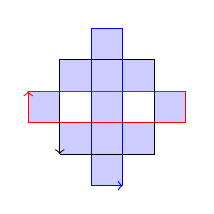
\begin{tikzpicture}[fill=blue!20,scale=0.4] 
\fill (0,2) -- (0,3) -- (5,3) -- (5,2) 
	  (2,0) -- (3,0) -- (3,5) -- (2,5)
	  (1,1) -- (4,1) -- (4,4) -- (1,4); 
\draw[red,->]
(0,3) -- (5,3) -- (5,2) -- (0,2) -- (0,3); 
\draw[blue,->]
(3,0) -- (3,5) -- (2,5) -- (2,0) -- (3,0); 
\draw[->]
(1,1) -- (4,1) -- (4,4) -- (1,4) -- (1,1); 
\end{tikzpicture} \\
\vspace{5mm}
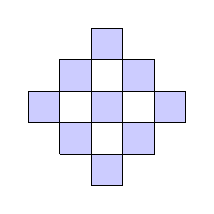
\begin{tikzpicture}[fill=blue!20,scale=0.4] 
\fill[even odd rule]
(0,2) -- (0,3) -- (5,3) -- (5,2)
(2,0) -- (3,0) -- (3,5) -- (2,5)
(1,1) -- (4,1) -- (4,4) -- (1,4);
\draw (0,3) -- (5,3) -- (5,2) -- (0,2) -- (0,3);
\draw (3,0) -- (3,5) -- (2,5) -- (2,0) -- (3,0); 
\draw (1,1) -- (4,1) -- (4,4) -- (1,4) -- (1,1); 
\end{tikzpicture}
\column{8cm}
\scriptsize
\begin{lstlisting}

\begin{tikzpicture}[scale=0.4,fill=gray] 
\path[fill] (0,0) rectangle (1,1); 
\path[fill=black!30] (2,0) -- (3,0) -- (3,1) -- cycle; 
\path[fill,color=gray] (4,0) -- (5,0) -- (5,1); 
\end{tikzpicture} 
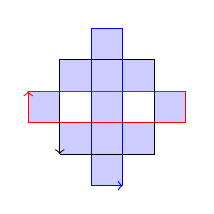
\begin{tikzpicture}[fill=blue!20,scale=0.4] 
\fill (0,2) -- (0,3) -- (5,3) -- (5,2) 
	  (2,0) -- (3,0) -- (3,5) -- (2,5)
	  (1,1) -- (4,1) -- (4,4) -- (1,4); 
\draw[red,->] (0,3) -- (5,3) -- (5,2) -- (0,2) -- (0,3); 
\draw[blue,->] (3,0) -- (3,5) -- (2,5) -- (2,0) -- (3,0); 
\draw[->] (1,1) -- (4,1) -- (4,4) -- (1,4) -- (1,1); 
\end{tikzpicture}
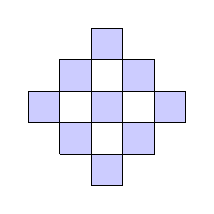
\begin{tikzpicture}[fill=blue!20,scale=0.4] 
\fill[even odd rule]
(0,2) -- (0,3) -- (5,3) -- (5,2)
(2,0) -- (3,0) -- (3,5) -- (2,5)
(1,1) -- (4,1) -- (4,4) -- (1,4);
\draw (0,3) -- (5,3) -- (5,2) -- (0,2) -- (0,3);
\draw (3,0) -- (3,5) -- (2,5) -- (2,0) -- (3,0); 
\draw (1,1) -- (4,1) -- (4,4) -- (1,4) -- (1,1); 
\end{tikzpicture}
\end{lstlisting}
\end{columns}
\end{frame}

\begin{frame}
\frametitle{Linije, strelice}
\begin{columns}
\column{3cm}
\tikz \draw[line width=8pt] (0,0) -- (2,4pt);
\tikz \draw[dash pattern=on 4mm off 1mm on 4mm off 2mm] (0,0.5) -- (2,0.5);

\tikz \draw[dash pattern=on 3mm off 2mm on 3mm off 3mm] (0,0.0) -- (2,0.0);	

\begin{tikzpicture}[dash pattern=on 3mm off 2mm] 
\draw[dash phase=3mm] (0,0.5) -- (2,0.5); 
\draw[dash phase=2mm] (0,0.0) -- (2,0.0); 
\end{tikzpicture}

\vspace{1cm}

\begin{tikzpicture}[line width=8pt] 
\draw[line join=round] (0.0,.8)--(0.3,.0)--(0.6,.8); 
\draw[line join=miter] (0.9,.0)--(1.2,.8)--(1.5,.0); 
\draw[line join=bevel] (1.8,.8)--(2.1,.0)--(2.4,.8); 
\end{tikzpicture}
\tikz \draw[->] (0,1.0) -- (2,1.0); 
\tikz \draw[<-] (0,0.5) -- (2,0.5); 
\tikz \draw[<->] (0,0.0) -- (2,0.0);
\tikz \draw[>=o,<->] (0,1.0) -- (2,1.0); 
\tikz \draw[>=*,<-] (0,0.5) -- (2,0.5); 
\tikz \draw[>=latex,->] (0,0.0) -- (2,0.0);
\column{7cm}
Predefinirane vrste linija:

\texttt{ultra thin} \tikz \draw[ultra thin] (0,0) -- (2,0); \\
\texttt{very thin} \tikz \draw[very thin] (0,0) -- (2,0); \\
\texttt{thin} \tikz \draw[thin] (0,0) -- (2,0); \\
\texttt{semithick} \tikz \draw[semithick] (0,0) -- (2,0); \\
\texttt{thick} \tikz \draw[thick] (0,0) -- (2,0); \\
\texttt{very thick} \tikz \draw[very thick] (0,0) -- (2,0); \\
\texttt{ultra thick} \tikz \draw[ultra thick] (0,0) -- (2,0); \\
\texttt{loosely dotted} \tikz \draw[loosely dotted] (0,0) -- (2,0); \\
\texttt{dotted} \tikz \draw[dotted] (0,0) -- (2,0); \\
\texttt{densely dotted} \tikz \draw[densely dotted] (0,0) -- (2,0); \\
\texttt{solid} \tikz \draw[solid] (0,0) -- (2,0); \\
\texttt{loosely dashed} \tikz \draw[loosely dashed] (0,0) -- (2,0); \\
\texttt{dashed} \tikz \draw[dashed] (0,0) -- (2,0); \\
\texttt{densely dashed} \tikz \draw[densely dashed] (0,0) -- (2,0); \\
\end{columns}
\end{frame}

\begin{frame}[fragile]
\frametitle{K\^odovi za prethodni slajd (lijeva strana)}
\scriptsize
\begin{lstlisting}
\tikz \draw[line width=8pt] (0,0) -- (2,4pt);
\tikz \draw[dash pattern=on 4mm off 1mm on 4mm off 2mm] (0,0.5) -- (2,0.5);

\tikz \draw[dash pattern=on 3mm off 2mm on 3mm off 3mm] (0,0.0) -- (2,0.0);	

\begin{tikzpicture}[dash pattern=on 3mm off 2mm] 
\draw[dash phase=3mm] (0,0.5) -- (2,0.5); 
\draw[dash phase=2mm] (0,0.0) -- (2,0.0); 
\end{tikzpicture}

\vspace{1cm}

\begin{tikzpicture}[line width=8pt] 
\draw[line join=round] (0.0,.8)--(0.3,.0)--(0.6,.8); 
\draw[line join=miter] (0.9,.0)--(1.2,.8)--(1.5,.0); 
\draw[line join=bevel] (1.8,.8)--(2.1,.0)--(2.4,.8); 
\end{tikzpicture}
\tikz \draw[->] (0,1.0) -- (2,1.0); 
\tikz \draw[<-] (0,0.5) -- (2,0.5); 
\tikz \draw[<->] (0,0.0) -- (2,0.0);
\tikz \draw[>=o,<->] (0,1.0) -- (2,1.0); 
\tikz \draw[>=*,<-] (0,0.5) -- (2,0.5); 
\tikz \draw[>=latex,->] (0,0.0) -- (2,0.0);	
\end{lstlisting}
\end{frame}

\begin{frame}[fragile]
\frametitle{Označavanje}
\begin{columns}
\column{55mm}
\small

\begin{tikzpicture}
\draw (0,0) node(oznaka)[scale=1.25] {Oznaka}; 
\draw (oznaka.north) circle (2pt)
node[anchor=south] {sjever}; 
\draw (oznaka.north east) circle (2pt)
node[anchor=south west] {sjeveroistok};
\draw (oznaka.north west) circle (2pt)
node[anchor=south east] {sjeverozapad};
\draw (oznaka.south) circle (2pt)
node[anchor=north] {jug};
\draw (oznaka.south east) circle (2pt)
node[anchor=north west] {jugoistok};
\draw (oznaka.south west) circle (2pt)
node[anchor=north east] {jugozapad};
\draw (oznaka.west) circle (2pt)
node[anchor=east] {zapad};
\draw (oznaka.east) circle (2pt)
node[anchor=west] {istok};
\end{tikzpicture}  
\column{65mm}
\scriptsize
\begin{lstlisting}
\draw (0,0) node(oznaka)[scale=1.25] {Oznaka}; 
\draw (oznaka.north) circle (2pt)
node[anchor=south] {sjever}; 
\draw (oznaka.north east) circle (2pt)
node[anchor=south west] {sjeveroistok};
\draw (oznaka.north west) circle (2pt)
node[anchor=south east] {sjeverozapad};
\draw (oznaka.south) circle (2pt)
node[anchor=north] {jug};
\draw (oznaka.south east) circle (2pt)
node[anchor=north west] {jugoistok};
\draw (oznaka.south west) circle (2pt)
node[anchor=north east] {jugozapad};
\draw (oznaka.west) circle (2pt)
node[anchor=east] {zapad};
\draw (oznaka.east) circle (2pt)
node[anchor=west] {istok};	
\end{lstlisting}
\end{columns}
\end{frame}

\begin{frame}[fragile]
\frametitle{Označavanje}
\begin{columns}
\column{25mm}    
\tikz \fill[fill=yellow!80!black]
      (0,0) node{prva}
   -- (1,1) node[ellipse,draw] {druga}
   -- (0,2) node[circle,fill=red!20] {treća}; \\
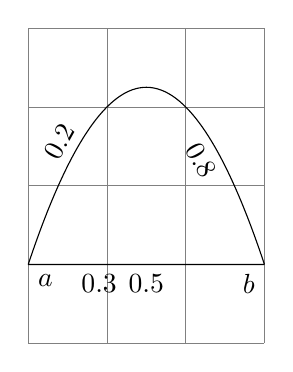
\begin{tikzpicture}
\draw[help lines] (0,0) grid (3,4); 
\draw (0,1) coordinate(a)
node[anchor=north west] {$a$} -- (3,1) coordinate(b)
node[anchor=north east] {$b$} 
node[pos=0.3,anchor=north] {$0.3$} 
node[pos=0.5,anchor=north] {$0.5$}
(a) .. controls (1,4) and (2,4) .. (b) 
node[pos=0.2,sloped,anchor=south] {$0.2$} 
node[pos=0.8,sloped,anchor=north] {$0.8$};     
\end{tikzpicture}
\column{7cm}
\scriptsize
\begin{lstlisting}
\tikz \fill[fill=yellow!80!black]
      (0,0) node{prva}
   -- (1,1) node[ellipse,draw] {druga}
   -- (0,2) node[circle,fill=red!20] {treća};\\
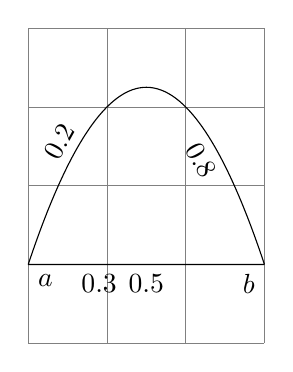
\begin{tikzpicture}
\draw[help lines] (0,0) grid (3,4); 
\draw (0,1) coordinate(a)
node[anchor=north west] {$a$} -- (3,1) coordinate(b)
node[anchor=north east] {$b$} 
node[pos=0.3,anchor=north] {$0.3$} 
node[pos=0.5,anchor=north] {$0.5$}
(a) .. controls (1,4) and (2,4) .. (b) 
node[pos=0.2,sloped,anchor=south] {$0.2$} 
node[pos=0.8,sloped,anchor=north] {$0.8$};     
\end{tikzpicture}  
\end{lstlisting}
\end{columns}    
\end{frame}

\begin{frame}[fragile]
\frametitle{Označavanje}  
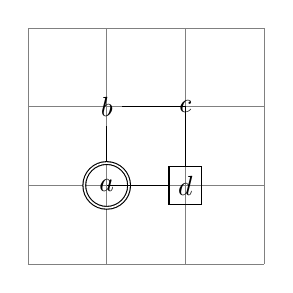
\begin{tikzpicture}
\draw[help lines] (0,0) grid (3,3);
\path (1,1) node(a)[draw,shape=circle,double] {$a$};
\path (1,2) node(b)[shape=rectangle] {$b$};
\path (2,2) node(c)[shape=circle] {$c$};
\path (2,1) node(d)[draw,shape=rectangle] {$d$}; 
\draw (a) -- (b) -- (c.center) -- (d) -- (a.center);  
\end{tikzpicture} 
\tikz \draw (0,0) node[ellipse split,draw] {g \nodepart{lower} d};

\begin{lstlisting}
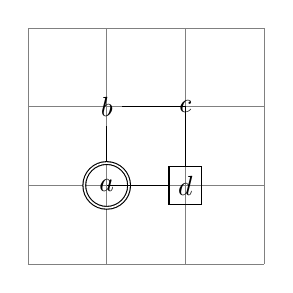
\begin{tikzpicture}
\draw[help lines] (0,0) grid (3,3);
\path (1,1) node(a)[draw,shape=circle,double] {$a$};
\path (1,2) node(b)[shape=rectangle] {$b$};
\path (2,2) node(c)[shape=circle] {$c$};
\path (2,1) node(d)[draw,shape=rectangle] {$d$}; 
\draw (a) -- (b) -- (c.center) -- (d) -- (a.center);  
\end{tikzpicture} \\
\tikz \draw (0,0) node[ellipse split,draw] {g \nodepart{lower} d};
\end{lstlisting} 
\end{frame}

\begin{frame}[fragile]
\frametitle{pic, angles}  
\textcolor{violet}{pic} je naredba koja omogućuje kreiranje \enquote{malih} slika koje se mogu ubaciti bilo gdje u Ti\emph{k}Z slici gdje možemo staviti  \textcolor{violet}{node}. Razlika je što \textcolor{violet}{pic} može biti puno kompleksniji objekt. U donjem kodu koristimo i \textcolor{violet}{angles} Ti\emph{k}Z biblioteku.
\begin{columns}
\column{30mm}
\begin{tikzpicture}
  \draw
  (3,-1) coordinate (a) node[right] {a}
  -- (0,0) coordinate (b) node[left] {b}
  -- (2,2) coordinate (c) node[above right] {c}
  pic["$\alpha$",draw=orange,<->,angle eccentricity=1.2,angle radius=1cm] {angle=a--b--c};  
\end{tikzpicture}
\column{80mm}
\small
\begin{lstlisting}
  \draw
  (3,-1) coordinate (a) node[right] {a}
  -- (0,0) coordinate (b) node[left] {b}
  -- (2,2) coordinate (c) node[above right] {c}
  pic["$\alpha$",draw=orange,<->,
  angle eccentricity=1.2,
  angle radius=1cm] {angle=a--b--c}; 
\end{lstlisting}
\end{columns}
\end{frame}

\begin{frame}[fragile]
\frametitle{Biblioteka \textcolor{violet}{spy}}
\begin{columns}
\column{30mm}
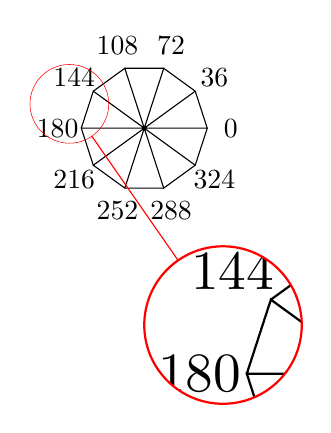
\begin{tikzpicture}
[spy using outlines={circle,
magnification=2, size=2cm, connect spies}]
\draw (-36:0.8)
\foreach \angle in {0,36,...,359} {
-- (\angle:0.8)
(\angle:1.1) node {$\angle$} 
(0,0) -- (\angle:0.8)
};
\spy[red] on (162:1.0) in node[right] at (0,-2.5); 
\end{tikzpicture}    
\column{78mm}
\small
\begin{lstlisting}
[spy using outlines={circle,
magnification=2, size=2cm, connect spies}]
\draw (-36:0.8)
\foreach \angle in {0,36,...,359} {
-- (\angle:0.8)
(\angle:1.1) node {$\angle$} 
(0,0) -- (\angle:0.8)
};
\spy[red] on (162:1.0) in node[right] at (0,-2.5); 
\end{lstlisting}
\end{columns}
\end{frame}

\begin{frame}[fragile]
\frametitle{Stabla}
\begin{columns}
\column{30mm}
\begin{tikzpicture}
[level 2/.style={sibling distance=10mm}]
\node {$f_4$}
child {node {$f_3$}
child {node {$f_2$}
child {node {$f_1$}}
child {node {$f_0$}}} child {node {$f_1$}}}
child {node {$f_2$}
child {node {$f_1$}}
child {node {$f_0$}}}; 
\end{tikzpicture}    
\column{78mm}
\small
\begin{lstlisting}
\begin{tikzpicture}
  [level 2/.style={sibling distance=10mm}]
\node {$f_4$}
  child {node {$f_3$}
    child {node {$f_2$}
      child {node {$f_1$}}
      child {node {$f_0$}}} 
    child {node {$f_1$}}}
  child {node {$f_2$}
    child {node {$f_1$}}
    child {node {$f_0$}}}; 
\end{tikzpicture}  
\end{lstlisting}
\end{columns}    
\end{frame}

\begin{frame}[fragile]
\frametitle{Stabla s oznakama}
\begin{columns}
\column{30mm}
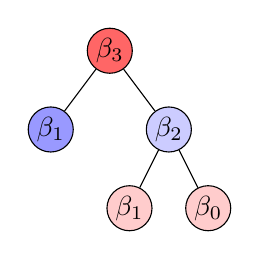
\begin{tikzpicture}
[level distance=10mm%
,every node/.style={fill=red!60,% 
                    circle,%
                    draw=black,%
                    inner sep=1pt}% 
,level 1/.style={sibling distance=15mm},%
,level 2/.style={sibling distance=10mm,% 
              nodes={fill=red!20}}]
\node (top) {$\beta_3$}
child {node[fill=blue!40] {$\beta_1$}} 
child {node[fill=blue!20] {$\beta_2$}
    child {node {$\beta_1$}}
    child {node {$\beta_0$}}}; 
\end{tikzpicture} 
\column{78mm}
\small
\begin{lstlisting}
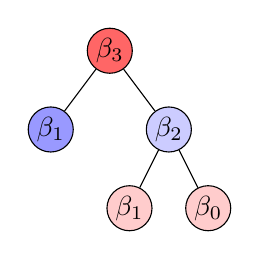
\begin{tikzpicture}
[level distance=10mm%
,every node/.style={fill=red!60,% 
                    circle,%
                    draw=black,%
                    inner sep=1pt}% 
,level 1/.style={sibling distance=15mm},%
,level 2/.style={sibling distance=10mm,% 
              nodes={fill=red!20}}]
\node (top) {$\beta_3$}
child {node[fill=blue!40] {$\beta_1$}} 
child {node[fill=blue!20] {$\beta_2$}
    child {node {$\beta_1$}}
    child {node {$\beta_0$}}}; 
\end{tikzpicture}
\end{lstlisting}
\end{columns}    
\end{frame}

\begin{frame}[fragile]
\frametitle{Stabla -- nedostajuća djeca}
\begin{columns}
\column{30mm}
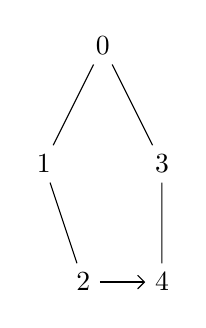
\begin{tikzpicture}
    [level 2/.style={sibling distance=10mm}]
\node (top) {$0$}
    child {node {$1$}
    child[missing]
child {node {$2$}}} 
    child {node {$3$}
        child {node {$4$}}}; 
\draw[-angle 90]
    (top-1-2.east) -- (top-2-1.west); 
\end{tikzpicture}
\column{78mm}
\small
\begin{lstlisting}
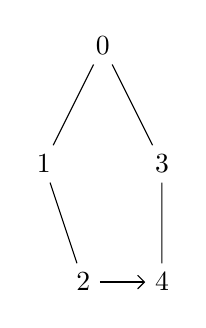
\begin{tikzpicture}
    [level 2/.style={sibling distance=10mm}]
\node (top) {$0$}
    child {node {$1$}
    child[missing]
child {node {$2$}}} 
    child {node {$3$}
        child {node {$4$}}}; 
\draw[-angle 90]
    (top-1-2.east) -- (top-2-1.west); 
\end{tikzpicture}
\end{lstlisting}
\end{columns}    
\end{frame}

\begin{frame}[fragile]
\frametitle{Koordinatni sustavi}
\begin{columns}
\column{30mm}
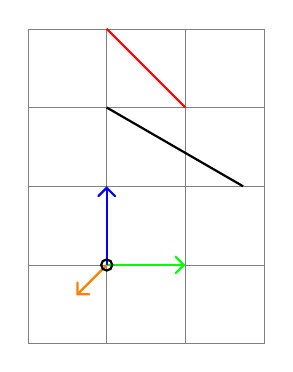
\begin{tikzpicture}[>=angle 90,thick] 
\draw[help lines] (-1,-1) grid (2,3); 
\draw[red] (canvas cs:x=1cm,y=2cm) -- (0,3); 
\draw[green,->] (0,0) -- (xyz cs:x=1,y=0,z=0); 
\draw[blue,->] (0,0) -- (0,1,0); 
\draw[orange,->] (0,0) -- (0,0,1);
\draw (canvas polar cs:radius=2cm,angle=30) 
                -- (90:2);
\path (0,0) coordinate (origin); 
\draw (origin) circle (2pt); 
\end{tikzpicture}
\column{78mm}
\small
\begin{lstlisting}
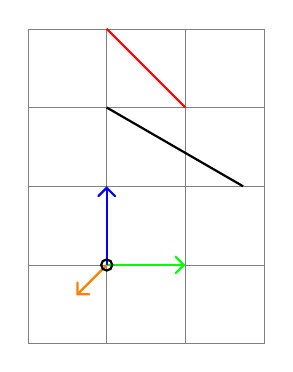
\begin{tikzpicture}[>=angle 90,thick] 
\draw[help lines] (-1,-1) grid (2,3); 
\draw[red] (canvas cs:x=1cm,y=2cm) -- (0,3); 
\draw[green,->] (0,0) -- (xyz cs:x=1,y=0,z=0); 
\draw[blue,->] (0,0) -- (0,1,0); 
\draw[orange,->] (0,0) -- (0,0,1);
\draw (canvas polar cs:radius=2cm,angle=30)
                -- (90:2);
\path (0,0) coordinate (origin); 
\draw (origin) circle (2pt); 
\end{tikzpicture}
\end{lstlisting}
\end{columns}  
\begin{block}{Vrste koordinatnih sustava}
eksplicitni <ime sustava> cs: <specifikacija koordinata>\\
implicitni (0,1),(label),(0,1 |- label),....  
\end{block}
\end{frame}

\begin{frame}[fragile]
\frametitle{Relativne i inkrementalne koordinate}
\begin{columns}
\column{30mm}
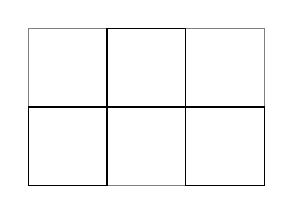
\begin{tikzpicture}
\draw[help lines] (0,0) grid +(3,2);
\draw (0,0) -- (+1,0) --
      (1,1) -- (+0,1) --cycle;  
\draw (1,1) -- +(1,0) --
      +(1,1) -- +(+0,1) -- cycle; 
\draw (2,0) -- ++(+1,0) --
    ++(0,1) -- ++(-1,0) -- cycle;  
\end{tikzpicture}
\column{78mm}
\small
\begin{lstlisting}
\draw[help lines] (0,0) grid +(3,2);
\draw (0,0) -- (+1,0) --
      (1,1) -- (+0,1) --cycle;  
\draw (1,1) -- +(1,0) --
      +(1,1) -- +(+0,1) -- cycle; 
\draw (2,0) -- ++(+1,0) --
    ++(0,1) -- ++(-1,0) -- cycle; 
\end{lstlisting}
\end{columns}
\begin{description}
  \item[Relativne koordinate] Konstruira nove koordinate ne mijenjajući trenutne koordinate. Notacija je \textcolor{violet}{+<pomak>}.
  \item[Inkrementalne koordinate] Isto kao i relative koordinate, ali sada se mijenjaju trenutne koordinate. Notacija je \textcolor{violet}{++<pomak>}.
\end{description}    
\end{frame}

\begin{frame}[fragile]
\frametitle{Računanja s koordinatama -- biblioteka \textcolor{violet}{calc}}
\framesubtitle{Projekcije}
\begin{columns}
\column{30mm}
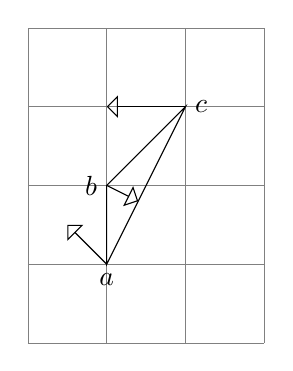
\begin{tikzpicture}[>=open triangle 90]
\draw[help lines] (0,0) grid +(3,4);
\draw (1,1) coordinate(a) node[anchor=north] {$a$}
-- (1,2) coordinate(b) node[anchor=east] {$b$} 
-- (2,3) coordinate(c) node[anchor=west] {$c$} 
-- cycle;
\draw[->] (b) -- ($(a)!(b)!(c)$); 
\draw[->] (c) -- ($(b)!(c)!(a)$); 
\draw[->] (a) -- ($(c)!(a)!(b)$); 
\end{tikzpicture}
\column{80mm}
\small
\begin{lstlisting}
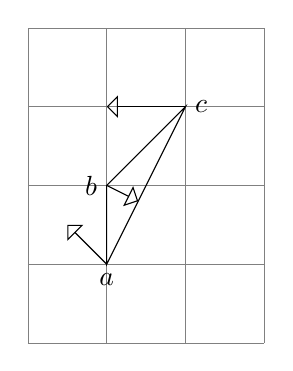
\begin{tikzpicture}[>=open triangle 90]
\draw[help lines] (0,0) grid +(3,4);
\draw (1,1) coordinate(a) node[anchor=north] {$a$}
-- (1,2) coordinate(b) node[anchor=east] {$b$} 
-- (2,3) coordinate(c) node[anchor=west] {$c$} 
-- cycle;
\draw[->] (b) -- ($(a)!(b)!(c)$); 
\draw[->] (c) -- ($(b)!(c)!(a)$); 
\draw[->] (a) -- ($(c)!(a)!(b)$); 
\end{tikzpicture}
\end{lstlisting}
\end{columns}
Općenita sintaksa je \textcolor{violet}{([<opcije>]\$<račun s koordinatama>\$)}. U slučaju računanja projekcija $(a)!(b)!(c)$ računa projekciju od $b$ na pravac kroz točke $a$ i $c$. Račun može biti i bitno kompliciraniji, a postoje i druge operacije.   
\end{frame}

\begin{frame}[fragile]
\frametitle{Definiranje stilova}
\begin{center}
\tikzset{Croatia/.style={red,dashed,thick}} 
\tikz \draw[Croatia] (0,0) rectangle (1,1);    
\tikzset{thick dashed/.style={thick,dashed}} 
\qquad
\begin{tikzpicture}[help lines/.style={ultra thin,blue!60}] 
\draw[thick dashed] (0,0) rectangle (1,1);
\draw[help lines] (1,1) rectangle (2,2);
\end{tikzpicture}
\end{center}
\begin{lstlisting}
\tikzset{Croatia/.style={red,dashed,thick}} 
\tikz \draw[Croatia] (0,0) rectangle (1,1);    
\tikzset{thick dashed/.style={thick,dashed}} 
\qquad
\begin{tikzpicture}[help lines/.style={ultra thin,blue!60}] 
\draw[thick dashed] (0,0) rectangle (1,1);
\draw[help lines] (1,1) rectangle (2,2);
\end{tikzpicture}  
\end{lstlisting}
\end{frame}

\begin{frame}[fragile]
\frametitle{Definiranje stilova}
\begin{center}
\tikzset{ seagull/.pic={
    \draw (-3mm,0) to [bend left] (0,0) to [bend left] (3mm,0);
  }
}
\begin{tikzpicture}
\fill [fill=blue!20] (1,1)
-- (2,2) pic {seagull} -- (3,2) pic {seagull} -- (3,1) pic [rotate=30] {seagull} -- (2,1) pic [red] {seagull};
\end{tikzpicture}
\end{center}
\begin{lstlisting}
\tikzset{ seagull/.pic={
    \draw (-3mm,0) to [bend left] (0,0) to [bend left] (3mm,0);
  }
}
\begin{tikzpicture}
\fill [fill=blue!20] (1,1)
-- (2,2) pic {seagull} -- (3,2) pic {seagull} -- (3,1) pic 
[rotate=30] {seagull} -- (2,1) pic [red] {seagull};
\end{tikzpicture}
\end{lstlisting}
\end{frame}

\begin{frame}[fragile]
\frametitle{\textcolor{violet}{scope} okolina, \textcolor{violet}{\textbackslash foreach}}
\begin{columns}
\column{30mm}
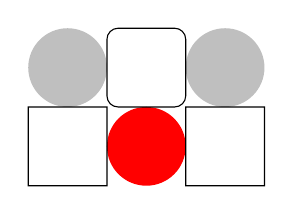
\begin{tikzpicture}
\begin{scope}[fill=gray!50]
  \fill (0.5,1.5) circle (0.5);
  \begin{scope}[fill=red]
    \fill (1.5,0.5) circle (0.5);        
  \end{scope}      
  \fill (2.5,1.5) circle (0.5);
\end{scope}  
\draw (0,0) rectangle (1,1)
      {[rounded corners] rectangle (2,2)}
      (2,1) rectangle (3,0);  
\end{tikzpicture} 

\begin{tikzpicture}
  \foreach \pos/\text in 
    {{0,0}/1, {1,0}/2, {1,1}/3, {0,1}/4} 
    { \draw (\pos) node {\text};}
\end{tikzpicture}
\column{80mm}
\small
\begin{lstlisting}
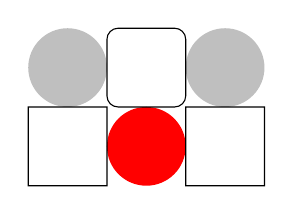
\begin{tikzpicture}
\begin{scope}[fill=gray!50]
  \fill (0.5,1.5) circle (0.5);
  \begin{scope}[fill=red]
    \fill (1.5,0.5) circle (0.5);        
  \end{scope}      
  \fill (2.5,1.5) circle (0.5);
\end{scope}  
\draw (0,0) rectangle (1,1)
      {[rounded corners] rectangle (2,2)}
      (2,1) rectangle (3,0);  
\end{tikzpicture} 

\begin{tikzpicture}
  \foreach \pos/\text in 
    {{0,0}/1, {1,0}/2, {1,1}/3, {0,1}/4} 
    { \draw (\pos) node {\text};}
\end{tikzpicture}
\end{lstlisting}
\end{columns} 
\end{frame}

\begin{frame}[fragile]
\frametitle{\textcolor{violet}{\textbackslash clip}, \textcolor{violet}{\textbackslash path \ldots to}}
\begin{columns}
\column{32mm}
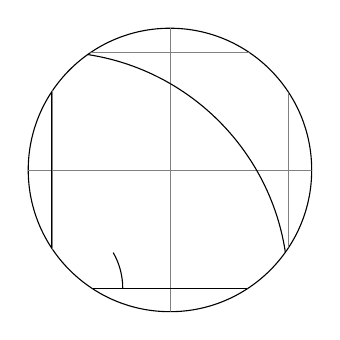
\begin{tikzpicture}[scale=3]
  \clip[draw] (0.5,0.5) circle (.6cm);
  \draw[step=.5cm,gray,very thin] (-1.4,-1.4) grid (1.4,1.4);
  \draw (-1.5,0) -- (1.5,0);
  \draw (0,-1.5) -- (0,1.5);
  \draw (0,0) circle (1cm);
  \draw (3mm,0mm) arc (0:30:3mm);
\end{tikzpicture} 
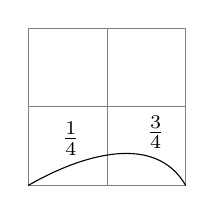
\begin{tikzpicture}
\draw[help lines] (0,0) grid (2,2);
\draw[out=30,in=120]
        (0,0) to node[pos=0.25,above] {$\frac{1}{4}$}
                 node[pos=0.75,above] {$\frac{3}{4}$}
                 (2,0);
\end{tikzpicture}
\tikzset{every to/.style={out=90,in=180}}
\begin{tikzpicture}
\draw[help lines] (0,0) to (2,2)
                  (0,0) to (1,1);
\end{tikzpicture}
\column{82mm}
\scriptsize
\begin{lstlisting}
\begin{tikzpicture}[scale=3]
  \clip[draw] (0.5,0.5) circle (.6cm);
  \draw[step=.5cm,gray,very thin] (-1.4,-1.4) grid (1.4,1.4);
  \draw (-1.5,0) -- (1.5,0);
  \draw (0,-1.5) -- (0,1.5);
  \draw (0,0) circle (1cm);
  \draw (3mm,0mm) arc (0:30:3mm);
\end{tikzpicture} 
\begin{tikzpicture}
\draw[help lines] (0,0) grid (2,2);
\draw[out=30,in=120]
        (0,0) to node[pos=0.25,above] {$\frac{1}{4}$}
                 node[pos=0.75,above] {$\frac{3}{4}$}
                 (2,0);
\end{tikzpicture}
\tikzset{every to/.style={out=90,in=180}}
\begin{tikzpicture}
\draw[help lines] (0,0) to (2,2)
                  (0,0) to (1,1);
\end{tikzpicture}
\end{lstlisting}
\end{columns} 
\end{frame}

\begin{frame}[fragile]
\frametitle{\textcolor{violet}{\textbackslash matrix}, \textcolor{violet}{opacity}}
\begin{columns}
\column{32mm}
\begin{tikzpicture}[every node/.style={midway}]
\matrix[column sep={4em,between origins},
row sep={2em}] at (0,0) {
\node(R) {$R$}; & \node(S) {$S$}; \\
\node(R/I) {$R/I$}; \\ 
};
\draw[->] (R)   -- (R/I) node[anchor=east]  {$\chi$};
\draw[->] (R/I) -- (S) node[anchor=north] {$\psi$};
\draw[->] (R)   -- (S) node[anchor=south] {$\phi$};
\end{tikzpicture}

\begin{tikzpicture}
\draw[clip] (0,0) circle (1cm);
\fill[blue,opacity=0.4] (1,0) circle (15mm);
\fill[red,opacity=0.3] (1,0) circle (1cm);
\end{tikzpicture}
\column{82mm}
\scriptsize
\begin{lstlisting}
\begin{tikzpicture}[every node/.style={midway}]
\matrix[column sep={4em,between origins},
row sep={2em}] at (0,0) {
\node(R) {$R$}; & \node(S) {$S$}; \\
\node(R/I) {$R/I$}; \\ 
};
\draw[->] (R)   -- (R/I) node[anchor=east]  {$\chi$};
\draw[->] (R/I) -- (S) node[anchor=north] {$\psi$};
\draw[->] (R)   -- (S) node[anchor=south] {$\phi$};
\end{tikzpicture}

\begin{tikzpicture}
\draw[clip] (0,0) circle (1cm);
\fill[blue,opacity=0.4] (1,0) circle (15mm);
\fill[red,opacity=0.3] (1,0) circle (1cm);
\end{tikzpicture}
\end{lstlisting}
\end{columns} 
\end{frame}

\begin{frame}
\frametitle{Kako je dobijen ovaj slajd?}
\tikzstyle{na} = [baseline=-.5ex]
\begin{flushleft}
\tikz[na,remember picture]{ 
\node[fill=blue!20,ellipse,anchor=base] (a) {4. travnja 2012.};
}
\end{flushleft}
  \begin{center}
    \tikz[na,remember picture]{ 
    \node[fill=blue!20,ellipse,anchor=base] (b) {\TeX nički Institut};
    }
\\          
          Certifikat
  \end{center}

  \noindent Potvrđuje se da je Pero Perić uspješno pohađao kurs na ovom Institutu i da je 
certificiran \TeX ničar.
  \begin{flushright}
    \tikz[na,remember picture]{ 
    \node[fill=blue!20,ellipse,anchor=base] (c) {Direktor \TeX ničkog Instituta};
    }
  \end{flushright}
Naredbe, tj. okoline su \textcolor{violet}{\textbackslash begin\{\smiley\} \ldots \textbackslash end\{\smiley\}} gdje je \\
\textcolor{violet}{\smiley} $=$
\tikz[baseline,remember picture] \node[anchor=base] (d) {\textcolor{violet}{flushleft},};
\tikz[baseline,remember picture] \node[anchor=base] (f) {\textcolor{violet}{center},};
\tikz[baseline,remember picture] \node[anchor=base] (e) {\textcolor{violet}{flushright}.};

\begin{tikzpicture}[remember picture,overlay]
  \path[->,red,very thick]<2-> (a) edge [bend right] (d);
  \path[->,red,very thick]<2-> (b) edge (f);
  \path[->,red,very thick]<2-> (c) edge [bend left] (e);
\end{tikzpicture}
\end{frame}

\begin{frame}[fragile]
\frametitle{\textcolor{violet}{overlay}, \textcolor{violet}{remember picture}}
\scriptsize
\begin{lstlisting}
\tikzstyle{na} = [baseline=-.5ex]
\begin{flushleft}
\tikz[na,remember picture]{ 
\node[fill=blue!20,ellipse,anchor=base] (a) {4. travnja 2012.};}
\end{flushleft}
  \begin{center}
    \tikz[na,remember picture]{ 
    \node[fill=blue!20,ellipse,anchor=base] (b) {\TeX nički Institut};}  
  \end{center}
\noindent Potvrđuje se da ...
  \begin{flushright}
    \tikz[na,remember picture]{ 
    \node[fill=blue!20,ellipse,anchor=base] (c) {Direktor \TeX ničkog Instituta};}
  \end{flushright}
Naredbe, tj. okoline su ...
\tikz[baseline,remember picture] \node[anchor=base] (d) {\textcolor{violet}{flushleft},};
\tikz[baseline,remember picture] \node[anchor=base] (f) {\textcolor{violet}{center},};
\tikz[baseline,remember picture] \node[anchor=base] (e) {\textcolor{violet}{flushright}.};
\begin{tikzpicture}[remember picture,overlay]
  \path[->,red,very thick]<2-> (a) edge [bend right] (d);
  \path[->,red,very thick]<2-> (b) edge (f);
  \path[->,red,very thick]<2-> (c) edge [bend left] (e);
\end{tikzpicture}      
\end{lstlisting}    
\end{frame}

\begin{frame}
\frametitle{Još o \textcolor{violet}{overlay}, \textcolor{violet}{remember picture} + \ldots}
\begin{tikzpicture}[remember picture,overlay]
  \node [rotate=60,scale=10,text opacity=0.3]
      at (current page.center) {Ti\textit{k}Z};
\end{tikzpicture}
\begin{tikzpicture}
  \filldraw[draw=black,fill=blue!20]
   plot [smooth,domain=0:1] (\x,{sqrt(\x)})
-- plot [smooth,domain=1:0] (\x,\x^2)
-- cycle; 
\end{tikzpicture} 
\begin{tikzpicture}
\draw (0,0,0)--(1,0,0)--(1,1,0)--(0,1,0)--cycle;
\draw (0,0,1)--(1,0,1)--(1,1,1)--(0,1,1)--cycle; 
\draw (0,0,0) -- (0,0,1); 
\draw (1,0,0) -- (1,0,1); 
\draw (1,1,0) -- (1,1,1); 
\draw (0,1,0) -- (0,1,1); 
\end{tikzpicture}
\hspace{2cm}
\begin{tikzpicture}
\draw [scale=0.25,rotate=45,ball color=pink]
(0,0) .. controls +(0,2)  and +(0,3)  .. (3,0)
      .. controls +(0,-2) and +(0,2)  .. (0,-4)
      .. controls +(0,2)  and +(0,-2) .. (-3,0)
      .. controls +(0,2)  and +(0,2)  .. (0,0);  
\end{tikzpicture} 
\end{frame}

\begin{frame}[fragile]
\frametitle{K\^od za prethodni slajd}
\scriptsize
\begin{lstlisting}
\begin{tikzpicture}[remember picture,overlay]
  \node [rotate=60,scale=10,text opacity=0.3]
      at (current page.center) {Ti\textit{k}Z};
\end{tikzpicture}
\begin{tikzpicture}
  \filldraw[draw=black,fill=blue!20]
   plot [smooth,domain=0:1] (\x,{sqrt(\x)})
-- plot [smooth,domain=1:0] (\x,\x^2) -- cycle; 
\end{tikzpicture} 
\begin{tikzpicture}
\draw (0,0,0)--(1,0,0)--(1,1,0)--(0,1,0)--cycle;
\draw (0,0,1)--(1,0,1)--(1,1,1)--(0,1,1)--cycle; 
\draw (0,0,0) -- (0,0,1); \draw (1,0,0) -- (1,0,1); 
\draw (1,1,0) -- (1,1,1); \draw (0,1,0) -- (0,1,1); 
\end{tikzpicture}
\begin{tikzpicture}
\draw [scale=0.25,rotate=45,ball color=pink]
(0,0) .. controls +(0,2)  and +(0,3)  .. (3,0)
      .. controls +(0,-2) and +(0,2)  .. (0,-4)
      .. controls +(0,2)  and +(0,-2) .. (-3,0)
      .. controls +(0,2)  and +(0,2)  .. (0,0);  
\end{tikzpicture} 
\end{lstlisting}     
\end{frame}

\begin{frame}[fragile]
\frametitle{matplotlib2tikz}
Skripta se može skinuti s \url{https://github.com/nschloe/matplotlib2tikz}.
\begin{block}{Što radi?}
A Python script for converting matplotlib figures into native Pgfplots (TikZ) figures.    
\end{block}    
Primjer upotrebe skripte.
\LaTeX{} k\^od:
\begin{lstlisting}
\usepackage{tikz}
\usepackage{pgfplots}
\pgfplotsset{compat=1.9}

\begin{center}
% This file was created by matplotlib v0.1.0.
% Copyright (c) 2010--2014, Nico Schlömer <nico.schloemer@gmail.com>
% All rights reserved.
% 
% The lastest updates can be retrieved from
% 
% https://github.com/nschloe/matplotlib2tikz
% 
% where you can also submit bug reports and leavecomments.
% 
\begin{tikzpicture}

\begin{axis}[
xmin=0, xmax=5,
ymin=-0.8, ymax=1,
axis on top,
xtick={0,1,2,3,4,5},
xticklabels={0,1,2,3,4,5}
]
\addplot [blue, mark=*, mark size=3, mark options={draw=black}, only marks]
coordinates {
(0,1)
(0.1,0.73202884833744)
(0.2,0.253001716518495)
(0.3,-0.228925419933261)
(0.4,-0.542300308913029)
(0.5,-0.606530659712633)
(0.6,-0.443997940310786)
(0.7,-0.153453298028392)
(0.8,0.138850285977112)
(0.9,0.328921764127384)
(1,0.367879441171442)
(1.1,0.269298363647752)
(1.2,0.0930741300882395)
(1.3,-0.0842169555549857)
(1.4,-0.199501134590026)
(1.5,-0.22313016014843)
(1.6,-0.163337714162804)
(1.7,-0.0564523135245992)
(1.8,0.051080165611755)
(1.9,0.121003554776307)
(2,0.135335283236613)
(2.1,0.0990693315271188)
(2.2,0.0342400589643796)
(2.3,-0.0309816865467285)
(2.4,-0.0733923659060474)
(2.5,-0.0820849986238988)
(2.6,-0.060088587008433)
(2.7,-0.0207676455522647)
(2.8,0.0187913427801971)
(2.9,0.044514720110866)
(3,0.0497870683678639)
(3.1,0.0364455703194248)
(3.2,0.0125962137574933)
(3.3,-0.0113975255333592)
(3.4,-0.0269995425557668)
(3.5,-0.0301973834223185)
(3.6,-0.0221053558094439)
(3.7,-0.00763998984021375)
(3.8,0.00691294868083993)
(3.9,0.0163760503582885)
(4,0.0183156388887342)
(4.1,0.0134075760422845)
(4.2,0.00463388807798266)
(4.3,-0.00419291532394942)
(4.4,-0.00993257662730005)
(4.5,-0.0111089965382423)
(4.6,-0.0081321059420741)
(4.7,-0.00281059519297333)
(4.8,0.00254313169755428)
(4.9,0.00602441225440258)

};
\addplot [black]
coordinates {
(0,1)
(0.02,0.972469513996579)
(0.04,0.930604472153162)
(0.06,0.875630518570151)
(0.08,0.808933020796294)
(0.1,0.73202884833744)
(0.12,0.646537173385705)
(0.14,0.554149794928787)
(0.16,0.456601475303023)
(0.18,0.3556407588801)
(0.2,0.253001716518495)
(0.22,0.150377027341965)
(0.24,0.0493927720726015)
(0.26,-0.0484147296565069)
(0.28,-0.141619751016491)
(0.3,-0.228925419933261)
(0.32,-0.309179222575896)
(0.34,-0.381385610807055)
(0.36,-0.444715627317404)
(0.38,-0.498513512820003)
(0.4,-0.542300308913029)
(0.42,-0.575774517305511)
(0.44,-0.598809920378729)
(0.46,-0.611450708933904)
(0.48,-0.613904099940109)
(0.5,-0.606530659712633)
(0.52,-0.589832575874769)
(0.54,-0.564440144426584)
(0.56,-0.531096756092869)
(0.58,-0.49064267876691)
(0.6,-0.443997940310787)
(0.62,-0.392144618302373)
(0.64,-0.336108840697778)
(0.66,-0.276942794041304)
(0.68,-0.215707024104248)
(0.7,-0.153453298028392)
(0.72,-0.0912082775993466)
(0.74,-0.0299582306302306)
(0.76,0.0293650179183697)
(0.78,0.0858967210123712)
(0.8,0.138850285977112)
(0.82,0.187526677838397)
(0.84,0.231322066127709)
(0.86,0.269733662821343)
(0.88,0.302363729806379)
(0.9,0.328921764127384)
(0.92,0.349224897827035)
(0.94,0.36319657604978)
(0.96,0.370863601871438)
(0.98,0.372351658736965)
(1,0.367879441171442)
(1.02,0.357751541365326)
(1.04,0.34235025316735)
(1.06,0.322126465844247)
(1.08,0.297589827635667)
(1.1,0.269298363647752)
(1.12,0.237847734041697)
(1.14,0.203860316883672)
(1.16,0.167974295572533)
(1.18,0.130832923634599)
(1.2,0.0930741300882398)
(1.22,0.0553206167835847)
(1.24,0.018170585387977)
(1.26,-0.017810783690502)
(1.28,-0.0520989948627857)
(1.3,-0.0842169555549857)
(1.32,-0.113740679623042)
(1.34,-0.140303925374529)
(1.36,-0.163601736457734)
(1.38,-0.183392872512635)
(1.4,-0.199501134590026)
(1.42,-0.211815607667108)
(1.44,-0.220289858876843)
(1.46,-0.224940145106487)
(1.48,-0.225842697218825)
(1.5,-0.22313016014843)
(1.52,-0.216987278397522)
(1.54,-0.20764592490638)
(1.56,-0.19537957783941)
(1.58,-0.18049735447963)
(1.6,-0.163337714162804)
(1.62,-0.144261943039465)
(1.64,-0.12364753248868)
(1.66,-0.101881560308373)
(1.68,-0.079354179484226)
(1.7,-0.0564523135245995)
(1.72,-0.0335536501934576)
(1.74,-0.0110210171427345)
(1.76,0.0108027863817992)
(1.78,0.0315996377244905)
(1.8,0.051080165611755)
(1.82,0.0689872094479267)
(1.84,0.0850986324176849)
(1.86,0.099229469143842)
(1.88,0.111233399951684)
(1.9,0.121003554776307)
(1.92,0.128472660255763)
(1.94,0.133612553432574)
(1.96,0.136433094607293)
(1.98,0.136980520135414)
(2,0.135335283236613)
(2.02,0.131609437115698)
(2.04,0.125943619820107)
(2.06,0.118503704241313)
(2.08,0.109477179488915)
(2.1,0.0990693315271188)
(2.12,0.0874992914831533)
(2.14,0.0749960194521983)
(2.16,0.0617942899863898)
(2.18,0.0481307428335222)
(2.2,0.0342400589643796)
(2.22,0.0203513175876046)
(2.24,0.0066845847982868)
(2.26,-0.00655222115088748)
(2.28,-0.0191661491157154)
(2.3,-0.0309816865467285)
(2.32,-0.0418428576581845)
(2.34,-0.0516149296609412)
(2.36,-0.0601857153827487)
(2.38,-0.0674664674547738)
(2.4,-0.0733923659060473)
(2.42,-0.0779226073799652)
(2.44,-0.0810401101793488)
(2.46,-0.0827508548787976)
(2.48,-0.0830828852455124)
(2.5,-0.0820849986238988)
(2.52,-0.0798251587181927)
(2.54,-0.0763886668160863)
(2.56,-0.0718761299118746)
(2.58,-0.0664012658988901)
(2.6,-0.060088587008433)
(2.62,-0.0530710029876651)
(2.64,-0.0454873851541632)
(2.66,-0.0374801314719188)
(2.68,-0.0291927712032753)
(2.7,-0.0207676455522647)
(2.72,-0.012343698082431)
(2.74,-0.00405440562760994)
(2.76,0.00397412301723084)
(2.78,0.0116248570673056)
(2.8,0.0187913427801971)
(2.82,0.0253789760596804)
(2.84,0.0313060373382718)
(2.86,0.0365044816563753)
(2.88,0.0409204810138249)
(2.9,0.0445147201108659)
(2.92,0.0472624504606988)
(2.94,0.0491533114902649)
(2.96,0.0501909306014215)
(2.98,0.0503923171987897)
(3,0.0497870683678639)
(3.02,0.0484164061790111)
(3.04,0.0463320684785294)
(3.06,0.0435950764930402)
(3.08,0.0402744036114078)
(3.1,0.0364455703194248)
(3.12,0.0321891904537196)
(3.14,0.0275894937261573)
(3.16,0.0227328488677791)
(3.18,0.0177063107767625)
(3.2,0.0125962137574933)
(3.22,0.00748683134123046)
(3.24,0.00245912132005687)
(3.26,-0.00241042745542018)
(3.28,-0.00705083222609791)
(3.3,-0.0113975255333592)
(3.32,-0.0153931270923092)
(3.34,-0.0189880714797703)
(3.36,-0.022141087341509)
(3.38,-0.0248195263450735)
(3.4,-0.0269995425557667)
(3.42,-0.0286661252575633)
(3.44,-0.0298129904452509)
(3.46,-0.0304423382492712)
(3.48,-0.0305644853950302)
(3.5,-0.0301973834223185)
(3.52,-0.0293660347806704)
(3.54,-0.0281018200601334)
(3.56,-0.0264417505055464)
(3.58,-0.02442766059196)
(3.6,-0.0221053558094439)
(3.62,-0.0195237309215102)
(3.64,-0.0167338738308637)
(3.66,-0.0137881698209217)
(3.68,-0.0107394203565067)
(3.7,-0.00763998984021375)
(3.72,-0.00454099275255374)
(3.74,-0.0014915324765675)
(3.76,0.00146199815472544)
(3.78,0.00427654592161826)
(3.8,0.00691294868083993)
(3.82,0.00933640353033871)
(3.84,0.0115168475212957)
(3.86,0.0134292483120005)
(3.88,0.0150538036878325)
(3.9,0.0163760503582885)
(3.92,0.0173868838638749)
(3.94,0.0180824927627645)
(3.96,0.0184642115015256)
(3.98,0.0185382974904248)
(4,0.0183156388887342)
(4.02,0.0178114004486642)
(4.04,0.0170446154601984)
(4.06,0.0160377323780859)
(4.08,0.0148161250940778)
(4.1,0.0134075760422846)
(4.12,0.0118417413958755)
(4.14,0.0101496075341818)
(4.16,0.00836294773771345)
(4.18,0.00651378771376335)
(4.2,0.00463388807798266)
(4.22,0.00275425132995676)
(4.24,0.000904660176995306)
(4.26,-0.000886746705284225)
(4.28,-0.00259385621913049)
(4.3,-0.00419291532394942)
(4.32,-0.0056628149925997)
(4.34,-0.00698532112490131)
(4.36,-0.00814525083812247)
(4.38,-0.00913059348196553)
(4.4,-0.00993257662730005)
(4.42,-0.010545678140303)
(4.44,-0.0109675862646485)
(4.46,-0.0111991103830939)
(4.48,-0.0112440458068164)
(4.5,-0.0111089965382423)
(4.52,-0.0108031604645342)
(4.54,-0.0103380818596223)
(4.56,-0.00972737639957511)
(4.58,-0.00898643412769592)
(4.6,-0.0081321059420741)
(4.62,-0.00718237922098678)
(4.64,-0.0061560481535316)
(4.66,-0.00507238420849761)
(4.68,-0.00395081195925693)
(4.7,-0.00281059519297333)
(4.72,-0.00167053787617307)
(4.74,-0.000548704133968712)
(4.76,0.000537839064154044)
(4.78,0.00157325332378893)
(4.8,0.00254313169755425)
(4.82,0.00343467091329208)
(4.84,0.00423681143019099)
(4.86,0.0049403443643713)
(4.88,0.00553798488818443)
(4.9,0.00602441225440258)
(4.92,0.00639627711955505)
(4.94,0.00665217733255245)
(4.96,0.00679260380885255)
(4.98,0.00681985852104743)

};
\path [draw=black, fill opacity=0] (axis cs:0,1)--(axis cs:5,1);

\path [draw=black, fill opacity=0] (axis cs:5,-0.8)--(axis cs:5,1);

\path [draw=black, fill opacity=0] (axis cs:0,-0.8)--(axis cs:5,-0.8);

\path [draw=black, fill opacity=0] (axis cs:0,-0.8)--(axis cs:0,1);

\end{axis}

\end{tikzpicture}
\end{center}  
\end{lstlisting}
\end{frame}

\begin{frame}[fragile]
\frametitle{matplotlib2tikz}
Python k\^od:
\begin{lstlisting}[language=Python]
import numpy as np
import matplotlib.pyplot as plt
def f(t):
    return np.exp(-t) * np.cos(2*np.pi*t)
t1 = np.arange(0.0, 5.0, 0.1)
t2 = np.arange(0.0, 5.0, 0.02)
fig = plt.figure();
fig, ax = plt.subplots();
ax.plot(t1, f(t1), 'bo', t2, f(t2), 'k'); 

from matplotlib2tikz import save as tikz_save
tikz_save('graf.tikz', figure=fig)
\end{lstlisting}

\end{frame}

\begin{frame}
\frametitle{matplotlib2tikz}
\begin{figure}
  \centering
  % This file was created by matplotlib v0.1.0.
% Copyright (c) 2010--2014, Nico Schlömer <nico.schloemer@gmail.com>
% All rights reserved.
% 
% The lastest updates can be retrieved from
% 
% https://github.com/nschloe/matplotlib2tikz
% 
% where you can also submit bug reports and leavecomments.
% 
\begin{tikzpicture}

\begin{axis}[
xmin=0, xmax=5,
ymin=-0.8, ymax=1,
axis on top,
xtick={0,1,2,3,4,5},
xticklabels={0,1,2,3,4,5}
]
\addplot [blue, mark=*, mark size=3, mark options={draw=black}, only marks]
coordinates {
(0,1)
(0.1,0.73202884833744)
(0.2,0.253001716518495)
(0.3,-0.228925419933261)
(0.4,-0.542300308913029)
(0.5,-0.606530659712633)
(0.6,-0.443997940310786)
(0.7,-0.153453298028392)
(0.8,0.138850285977112)
(0.9,0.328921764127384)
(1,0.367879441171442)
(1.1,0.269298363647752)
(1.2,0.0930741300882395)
(1.3,-0.0842169555549857)
(1.4,-0.199501134590026)
(1.5,-0.22313016014843)
(1.6,-0.163337714162804)
(1.7,-0.0564523135245992)
(1.8,0.051080165611755)
(1.9,0.121003554776307)
(2,0.135335283236613)
(2.1,0.0990693315271188)
(2.2,0.0342400589643796)
(2.3,-0.0309816865467285)
(2.4,-0.0733923659060474)
(2.5,-0.0820849986238988)
(2.6,-0.060088587008433)
(2.7,-0.0207676455522647)
(2.8,0.0187913427801971)
(2.9,0.044514720110866)
(3,0.0497870683678639)
(3.1,0.0364455703194248)
(3.2,0.0125962137574933)
(3.3,-0.0113975255333592)
(3.4,-0.0269995425557668)
(3.5,-0.0301973834223185)
(3.6,-0.0221053558094439)
(3.7,-0.00763998984021375)
(3.8,0.00691294868083993)
(3.9,0.0163760503582885)
(4,0.0183156388887342)
(4.1,0.0134075760422845)
(4.2,0.00463388807798266)
(4.3,-0.00419291532394942)
(4.4,-0.00993257662730005)
(4.5,-0.0111089965382423)
(4.6,-0.0081321059420741)
(4.7,-0.00281059519297333)
(4.8,0.00254313169755428)
(4.9,0.00602441225440258)

};
\addplot [black]
coordinates {
(0,1)
(0.02,0.972469513996579)
(0.04,0.930604472153162)
(0.06,0.875630518570151)
(0.08,0.808933020796294)
(0.1,0.73202884833744)
(0.12,0.646537173385705)
(0.14,0.554149794928787)
(0.16,0.456601475303023)
(0.18,0.3556407588801)
(0.2,0.253001716518495)
(0.22,0.150377027341965)
(0.24,0.0493927720726015)
(0.26,-0.0484147296565069)
(0.28,-0.141619751016491)
(0.3,-0.228925419933261)
(0.32,-0.309179222575896)
(0.34,-0.381385610807055)
(0.36,-0.444715627317404)
(0.38,-0.498513512820003)
(0.4,-0.542300308913029)
(0.42,-0.575774517305511)
(0.44,-0.598809920378729)
(0.46,-0.611450708933904)
(0.48,-0.613904099940109)
(0.5,-0.606530659712633)
(0.52,-0.589832575874769)
(0.54,-0.564440144426584)
(0.56,-0.531096756092869)
(0.58,-0.49064267876691)
(0.6,-0.443997940310787)
(0.62,-0.392144618302373)
(0.64,-0.336108840697778)
(0.66,-0.276942794041304)
(0.68,-0.215707024104248)
(0.7,-0.153453298028392)
(0.72,-0.0912082775993466)
(0.74,-0.0299582306302306)
(0.76,0.0293650179183697)
(0.78,0.0858967210123712)
(0.8,0.138850285977112)
(0.82,0.187526677838397)
(0.84,0.231322066127709)
(0.86,0.269733662821343)
(0.88,0.302363729806379)
(0.9,0.328921764127384)
(0.92,0.349224897827035)
(0.94,0.36319657604978)
(0.96,0.370863601871438)
(0.98,0.372351658736965)
(1,0.367879441171442)
(1.02,0.357751541365326)
(1.04,0.34235025316735)
(1.06,0.322126465844247)
(1.08,0.297589827635667)
(1.1,0.269298363647752)
(1.12,0.237847734041697)
(1.14,0.203860316883672)
(1.16,0.167974295572533)
(1.18,0.130832923634599)
(1.2,0.0930741300882398)
(1.22,0.0553206167835847)
(1.24,0.018170585387977)
(1.26,-0.017810783690502)
(1.28,-0.0520989948627857)
(1.3,-0.0842169555549857)
(1.32,-0.113740679623042)
(1.34,-0.140303925374529)
(1.36,-0.163601736457734)
(1.38,-0.183392872512635)
(1.4,-0.199501134590026)
(1.42,-0.211815607667108)
(1.44,-0.220289858876843)
(1.46,-0.224940145106487)
(1.48,-0.225842697218825)
(1.5,-0.22313016014843)
(1.52,-0.216987278397522)
(1.54,-0.20764592490638)
(1.56,-0.19537957783941)
(1.58,-0.18049735447963)
(1.6,-0.163337714162804)
(1.62,-0.144261943039465)
(1.64,-0.12364753248868)
(1.66,-0.101881560308373)
(1.68,-0.079354179484226)
(1.7,-0.0564523135245995)
(1.72,-0.0335536501934576)
(1.74,-0.0110210171427345)
(1.76,0.0108027863817992)
(1.78,0.0315996377244905)
(1.8,0.051080165611755)
(1.82,0.0689872094479267)
(1.84,0.0850986324176849)
(1.86,0.099229469143842)
(1.88,0.111233399951684)
(1.9,0.121003554776307)
(1.92,0.128472660255763)
(1.94,0.133612553432574)
(1.96,0.136433094607293)
(1.98,0.136980520135414)
(2,0.135335283236613)
(2.02,0.131609437115698)
(2.04,0.125943619820107)
(2.06,0.118503704241313)
(2.08,0.109477179488915)
(2.1,0.0990693315271188)
(2.12,0.0874992914831533)
(2.14,0.0749960194521983)
(2.16,0.0617942899863898)
(2.18,0.0481307428335222)
(2.2,0.0342400589643796)
(2.22,0.0203513175876046)
(2.24,0.0066845847982868)
(2.26,-0.00655222115088748)
(2.28,-0.0191661491157154)
(2.3,-0.0309816865467285)
(2.32,-0.0418428576581845)
(2.34,-0.0516149296609412)
(2.36,-0.0601857153827487)
(2.38,-0.0674664674547738)
(2.4,-0.0733923659060473)
(2.42,-0.0779226073799652)
(2.44,-0.0810401101793488)
(2.46,-0.0827508548787976)
(2.48,-0.0830828852455124)
(2.5,-0.0820849986238988)
(2.52,-0.0798251587181927)
(2.54,-0.0763886668160863)
(2.56,-0.0718761299118746)
(2.58,-0.0664012658988901)
(2.6,-0.060088587008433)
(2.62,-0.0530710029876651)
(2.64,-0.0454873851541632)
(2.66,-0.0374801314719188)
(2.68,-0.0291927712032753)
(2.7,-0.0207676455522647)
(2.72,-0.012343698082431)
(2.74,-0.00405440562760994)
(2.76,0.00397412301723084)
(2.78,0.0116248570673056)
(2.8,0.0187913427801971)
(2.82,0.0253789760596804)
(2.84,0.0313060373382718)
(2.86,0.0365044816563753)
(2.88,0.0409204810138249)
(2.9,0.0445147201108659)
(2.92,0.0472624504606988)
(2.94,0.0491533114902649)
(2.96,0.0501909306014215)
(2.98,0.0503923171987897)
(3,0.0497870683678639)
(3.02,0.0484164061790111)
(3.04,0.0463320684785294)
(3.06,0.0435950764930402)
(3.08,0.0402744036114078)
(3.1,0.0364455703194248)
(3.12,0.0321891904537196)
(3.14,0.0275894937261573)
(3.16,0.0227328488677791)
(3.18,0.0177063107767625)
(3.2,0.0125962137574933)
(3.22,0.00748683134123046)
(3.24,0.00245912132005687)
(3.26,-0.00241042745542018)
(3.28,-0.00705083222609791)
(3.3,-0.0113975255333592)
(3.32,-0.0153931270923092)
(3.34,-0.0189880714797703)
(3.36,-0.022141087341509)
(3.38,-0.0248195263450735)
(3.4,-0.0269995425557667)
(3.42,-0.0286661252575633)
(3.44,-0.0298129904452509)
(3.46,-0.0304423382492712)
(3.48,-0.0305644853950302)
(3.5,-0.0301973834223185)
(3.52,-0.0293660347806704)
(3.54,-0.0281018200601334)
(3.56,-0.0264417505055464)
(3.58,-0.02442766059196)
(3.6,-0.0221053558094439)
(3.62,-0.0195237309215102)
(3.64,-0.0167338738308637)
(3.66,-0.0137881698209217)
(3.68,-0.0107394203565067)
(3.7,-0.00763998984021375)
(3.72,-0.00454099275255374)
(3.74,-0.0014915324765675)
(3.76,0.00146199815472544)
(3.78,0.00427654592161826)
(3.8,0.00691294868083993)
(3.82,0.00933640353033871)
(3.84,0.0115168475212957)
(3.86,0.0134292483120005)
(3.88,0.0150538036878325)
(3.9,0.0163760503582885)
(3.92,0.0173868838638749)
(3.94,0.0180824927627645)
(3.96,0.0184642115015256)
(3.98,0.0185382974904248)
(4,0.0183156388887342)
(4.02,0.0178114004486642)
(4.04,0.0170446154601984)
(4.06,0.0160377323780859)
(4.08,0.0148161250940778)
(4.1,0.0134075760422846)
(4.12,0.0118417413958755)
(4.14,0.0101496075341818)
(4.16,0.00836294773771345)
(4.18,0.00651378771376335)
(4.2,0.00463388807798266)
(4.22,0.00275425132995676)
(4.24,0.000904660176995306)
(4.26,-0.000886746705284225)
(4.28,-0.00259385621913049)
(4.3,-0.00419291532394942)
(4.32,-0.0056628149925997)
(4.34,-0.00698532112490131)
(4.36,-0.00814525083812247)
(4.38,-0.00913059348196553)
(4.4,-0.00993257662730005)
(4.42,-0.010545678140303)
(4.44,-0.0109675862646485)
(4.46,-0.0111991103830939)
(4.48,-0.0112440458068164)
(4.5,-0.0111089965382423)
(4.52,-0.0108031604645342)
(4.54,-0.0103380818596223)
(4.56,-0.00972737639957511)
(4.58,-0.00898643412769592)
(4.6,-0.0081321059420741)
(4.62,-0.00718237922098678)
(4.64,-0.0061560481535316)
(4.66,-0.00507238420849761)
(4.68,-0.00395081195925693)
(4.7,-0.00281059519297333)
(4.72,-0.00167053787617307)
(4.74,-0.000548704133968712)
(4.76,0.000537839064154044)
(4.78,0.00157325332378893)
(4.8,0.00254313169755425)
(4.82,0.00343467091329208)
(4.84,0.00423681143019099)
(4.86,0.0049403443643713)
(4.88,0.00553798488818443)
(4.9,0.00602441225440258)
(4.92,0.00639627711955505)
(4.94,0.00665217733255245)
(4.96,0.00679260380885255)
(4.98,0.00681985852104743)

};
\path [draw=black, fill opacity=0] (axis cs:0,1)--(axis cs:5,1);

\path [draw=black, fill opacity=0] (axis cs:5,-0.8)--(axis cs:5,1);

\path [draw=black, fill opacity=0] (axis cs:0,-0.8)--(axis cs:5,-0.8);

\path [draw=black, fill opacity=0] (axis cs:0,-0.8)--(axis cs:0,1);

\end{axis}

\end{tikzpicture}
\end{figure}
\end{frame}

\begin{frame}
\frametitle{Okolina \textcolor{violet}{axis} iz paketa \textcolor{violet}{pgfplots}}
\begin{center}
\begin{tikzpicture}
\begin{axis}[width=8cm,height=6cm,tick align=outside]
\addplot[draw=blue]
coordinates {(0,1) (1,1) (2,3) (3,2) (4,2)};
\addlegendentry{Linija 1} 
\addplot[draw=red]
coordinates {(0,0) (1,4) (2,4) (3,3) (4,3)}; 
\addlegendentry{Linija 2}
\end{axis} 
\end{tikzpicture}
\end{center}
Paket \textcolor{violet}{pgfplots} smo već koristili kod uvoza slike iz Matlaba, no taj paket ima puno veće mogućnosti.
\end{frame}

\begin{frame}[fragile]
\frametitle{K\^od za prethodan slajd}
\begin{lstlisting}
\begin{tikzpicture}
\begin{axis}[width=8cm,height=6cm,tick align=outside]
\addplot[draw=blue]
coordinates {(0,1) (1,1) (2,3) (3,2) (4,2)};
\addlegendentry{Linija 1} 
\addplot[draw=red]
coordinates {(0,0) (1,4) (2,4) (3,3) (4,3)}; 
\addlegendentry{Linija 2}
\end{axis} 
\end{tikzpicture}  
\end{lstlisting}
\end{frame}

\begin{frame}
\frametitle{Grafikoni}
\begin{tikzpicture}
\begin{axis}
      [xbar stacked, stack plots=x, tick align=outside,
       width=8cm, height=6cm, bar width=10pt,
       legend style={cells={anchor=west}}, area legend,
       xlabel=\textbf{Osvojene medalje}, xtick={1,...,8},
       ytick={1,...,7}, yticklabels={Sjedinjene Američke Države, 
        Rusija, Grčka, Australija, Italija, Kanada, Mađarska}]
\addplot[draw=black,fill=yellow!50!brown]
        coordinates {(6,1) (1,2) (1,3) (0,4) (0,5) (0,6) (0,7)};
\addlegendentry{Zlato}
\addplot[draw=black,fill=white!60!gray]
        coordinates {(1,1) (1,2) (0,3) (2,4) (2,5) (1,6) (1,7)};
\addlegendentry{Srebro}
\addplot[draw=black,fill=orange!70!gray]
        coordinates {(0,1) (1,2) (2,3) (4,4) (1,5) (0,6) (0,7)};
\addlegendentry{Bronca}
\end{axis}      
\end{tikzpicture}    
\pause
\begin{block}{Bonus pitanje}
O kojem se sportu radi?
\end{block}
\end{frame}

\begin{frame}[fragile]
\frametitle{K\^od za prethodan slajd}
\small
\begin{lstlisting}
\begin{axis}
      [xbar stacked, stack plots=x, tick align=outside,
       width=8cm, height=6cm, bar width=10pt,
       legend style={cells={anchor=west}}, area legend,
       xlabel=\textbf{Osvojene medalje}, xtick={1,...,8},
       ytick={1,...,7}, yticklabels={Sjedinjene Američke Države, 
        Rusija, Grčka, Australija, Italija, Kanada, Mađarska}]
\addplot[draw=black,fill=yellow!50!brown]
        coordinates {(6,1) (1,2) (1,3) (0,4) (0,5) (0,6) (0,7)};
\addlegendentry{Zlato}
\addplot[draw=black,fill=white!60!gray]
        coordinates {(1,1) (1,2) (0,3) (2,4) (2,5) (1,6) (1,7)};
\addlegendentry{Srebro}
\addplot[draw=black,fill=orange!70!gray]
        coordinates {(0,1) (1,2) (2,3) (4,4) (1,5) (0,6) (0,7)};
\addlegendentry{Bronca}
\end{axis}       
\end{lstlisting}
\end{frame}

\begin{frame}
\frametitle{Raspršeni graf}
\begin{figure}
\centering  
\begin{tikzpicture}
\begin{axis}
      [width=8cm, height=7cm, tick align=outside,
       xlabel=\textbf{Postotak zaposlenih majki},
       ylabel=\textbf{Postotak siromašne djece}]
\addplot+[scatter,only marks,mark=triangle*,
         draw=blue,scatter src=explicit]
        file {mat_employ-child_pov.dat};
\draw[dashed,red!40]
     (rel axis cs:0,1) -- (rel axis cs:1,0);
\end{axis}  
\end{tikzpicture}
\caption{Prema OECDovom izvješću}
\end{figure}
\end{frame}

\begin{frame}[fragile]
\frametitle{K\^od za prethodan slajd}
\small
\begin{lstlisting}
\begin{tikzpicture}
\begin{axis}
      [width=8cm, height=7cm, tick align=outside,
       xlabel=\textbf{Postotak zaposlenih majki},
       ylabel=\textbf{Postotak siromašne djece}]
\addplot+[scatter,only marks,mark=triangle*,
         draw=blue,scatter src=explicit]
        file {mat_employ-child_pov.dat};
\draw[dashed,red!40]
     (rel axis cs:0,1) -- (rel axis cs:1,0);
\end{axis}  
\end{tikzpicture}  
\end{lstlisting}
Koordinatni sustavi:
\begin{description}
  \item[axis cs] Odgovara brojevima na osima.
  \item[rel axis cs] Relativne koordinate -- skalirane na kvadrat $[0,1]\times [0,1]$. 
  \item[xticklabel, yticklabel] Projekcije relativnih koordinata na osi.
\end{description}
\end{frame}

\begin{frame}
\frametitle{Dodatne naredbe i ostalo}
\begin{description}[<+->]
  \item[\textbackslash addplot+] Za dodavanje više grafova u jednu sliku.
  \item[\textbackslash pgfplotset] Analogon naredbe \textcolor{violet}{\textbackslash tikzset}, služi za predefiniranje vrijednosti na nivou cijelog dokumenta. 
  \item[datatool, pgfplotstable, spreadtab] Paketi za kreiranje baza podataka, crtanja grafikona i slično iz proračunskih tablica.
\end{description}
\end{frame}
\end{document}